\uuid{IjIT}
\exo7id{5782}
\auteur{rouget}
\organisation{exo7}
\datecreate{2010-10-16}
\isIndication{false}
\isCorrection{true}
\chapitre{Série de Fourier}
\sousChapitre{Calcul de coefficients}

\contenu{
\texte{
Développer en série de \textsc{Fourier} les fonctions suivantes puis déterminer la valeur des sommes indiquées :

\textbf{1) (**)} $f~:~\Rr\rightarrow\Rr$ $2\pi$-périodique paire telle que $\forall x\in[0,\pi]$, $f(x)=1-\frac{2x}{\pi}$. En déduire $\sum_{n=0}^{+\infty}\frac{1}{(2n+1)^2}$, $\sum_{n=1}^{+\infty}\frac{1}{n^2}$ et $\sum_{n=1}^{+\infty}\frac{1}{n^4}$.

\textbf{2) (**)} $f~:~\Rr\rightarrow\Rr$ $2\pi$-périodique impaire telle que $\forall x\in[0,\pi]$, $f(x)=x(\pi-x)$. En déduire $\sum_{n=0}^{+\infty}\frac{(-1)^n}{(2n+1)^3}$, $\sum_{n=0}^{+\infty}\frac{1}{(2n+1)^6}$ et $\sum_{n=1}^{+\infty}\frac{1}{n^6}$.

\textbf{3) (**)} $f~:~\Rr\rightarrow\Rr$ $2\pi$-périodique telle que $\forall x\in]-\pi,\pi]$, $f(x)=\sin\left(\frac{x}{2}\right)$. En déduire $\sum_{n=0}^{+\infty}(-1)^n\frac{2n+1}{16n^2+16n+3}$.

\textbf{4) (***)} $f~:~\Rr\rightarrow\Rr$ $2\pi$-périodique telle que $\forall x\in[-\pi,\pi]$, $f(x)=\ch(\lambda x)$ ($\lambda$ réel strictement positif donné). En déduire $\sum_{n=1}^{+\infty}\frac{(-1)^n}{\lambda^2+n^2}$, $\sum_{n=1}^{+\infty}\frac{1}{\lambda^2+n^2}$ et $\sum_{n=1}^{+\infty}\frac{1}{(\lambda^2+n^2)^2}$.

\textbf{5) (**)} $f~:~\Rr\rightarrow\Rr$ telle que $\forall x\in\Rr$, $f(x)=\text{sup}(0,\sin x)$. En déduire $\sum_{n=1}^{+\infty}\frac{1}{4p^2-1}$.
}
\reponse{
La fonction $f$ est continue par morceaux sur $\Rr$ et $2\pi$-périodique. On peut donc calculer ses coefficients de \textsc{Fourier}.

$$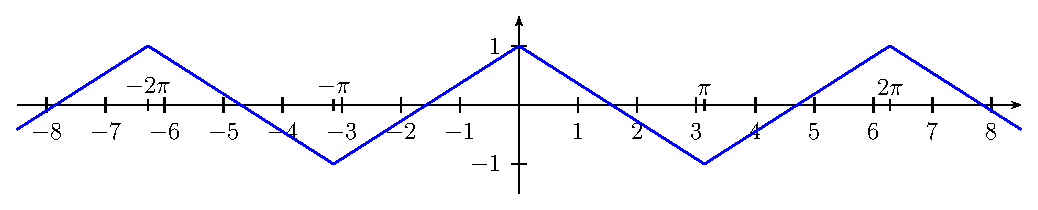
\includegraphics{../images/img005782-1}$$


Puisque $f$ est paire, $\forall n\in\Nn^*$, $b_n(f)=0$ puis pour $n\in\Nn$, $a_n(f)=\frac{2}{\pi}\int_{0}^{\pi}\left(1-\frac{2x}{\pi}\right)\cos(nx)\;dx$.

Par suite, $a_0(f)=0$ puis pour $n\in\Nn^*$,

\begin{center}
$a_n(f)=\frac{2}{\pi}\left(\left[\left(1-\frac{2x}{\pi}\right)\frac{\sin(nx)}{n}\right]_0^\pi+\frac{2}{n\pi}\int_{0}^{\pi}\sin(nx)\;dx\right)=\frac{4}{n\pi^2}\left[\frac{-\cos(nx)}{n}\right]_0^\pi=\frac{4(1-(-1)^n)}{n^2\pi^2}$.
\end{center} 

La fonction $f$ est $2\pi$-périodique, continue sur $\Rr$ et de classe $C^1$ par morceaux sur $\Rr$. D'après le théorème de \textsc{Dirichlet}, la série de \textsc{Fourier} de $f$ converge vers $f$ sur $\Rr$. Par suite, pour tout réel $x$, 

\begin{center}
$f(x)=\frac{a_0(f)}{2}+\sum_{n=1}^{+\infty}(a_n(f)\cos(nx)+b_n(f)\sin(nx))=\frac{4}{\pi^2}\sum_{n=1}^{+\infty}\frac{1-(-1)^n}{n^2}\cos(nx)=\frac{8}{\pi^2}\sum_{p=0}^{+\infty}\frac{\cos((2p+1)x)}{(2p+1)^2}$.
\end{center}

\begin{center}
\shadowbox{
$\forall x\in\Rr$, $f(x)=\frac{8}{\pi^2}\sum_{n=0}^{+\infty}\frac{\cos((2n+1)x)}{(2n+1)^2}$.
}
\end{center}

L'égalité $f(0)=1$ fournit $\sum_{n=0}^{+\infty}\frac{1}{(2n+1)^2}=\frac{\pi^2}{8}$. Ensuite, si $S=\sum_{n=1}^{+\infty}\frac{1}{n^2}$, on a

\begin{center}
$S=\sum_{n=0}^{+\infty}\frac{1}{(2n+1)^2}+\sum_{n=1}^{+\infty}\frac{1}{(2n)^2}=\frac{\pi^2}{8}+\frac{S}{4}$,
\end{center}

et donc $S=\frac{4}{3}\times\frac{\pi^2}{8}=\frac{\pi^2}{6}$.

D'autre part, puisque $f$ est continue par morceaux sur $\Rr$ et $2\pi$-périodique, la formule de \textsc{Parseval} fournit $\frac{(a_0(f))^2}{2}+\sum_{n=1}^{+\infty}((a_n(f))^2+(b_n(f))^2)=\frac{1}{\pi}\int_{-\pi}^{\pi}(f(x))^2\;dx$ et donc

\begin{center}
$\frac{64}{\pi^4}\sum_{n=0}^{+\infty}\frac{1}{(2n+1)^4}=\frac{2}{\pi}\int_{0}^{\pi}\left(1-\frac{2x}{\pi}\right)^2\;dx=\left[-\frac{1}{3}\left(1-\frac{2x}{\pi}\right)^3\right]_0^\pi=\frac{2}{3}$
\end{center}

et donc $\sum_{n=0}^{+\infty}\frac{1}{(2n+1)^4}=\frac{2}{3}\times\frac{\pi^4}{64}=\frac{\pi^4}{96}$. Enfin, si on pose $S=\frac{1}{n^4}$,

\begin{center}
$S=\sum_{n=0}^{+\infty}\frac{1}{(2n+1)^4}+\sum_{n=1}^{+\infty}\frac{1}{(2n)^4}=\frac{\pi^4}{96}+\frac{S}{16}$,
\end{center}

et donc $S=\frac{16}{15}\times\frac{\pi^4}{96}=\frac{\pi^4}{90}$.

\begin{center}
\shadowbox{
$\sum_{n=0}^{+\infty}\frac{1}{(2n+1)^2}=\frac{\pi^2}{8}$, $\sum_{n=1}^{+\infty}\frac{1}{n^2}=\frac{\pi^2}{6}$ et $\sum_{n=1}^{+\infty}\frac{1}{n^4}=\frac{\pi^4}{90}$.
}
\end{center}
La fonction $f$ est continue par morceaux sur $\Rr$ et $2\pi$-périodique. On peut donc calculer ses coefficients de \textsc{Fourier}.

$$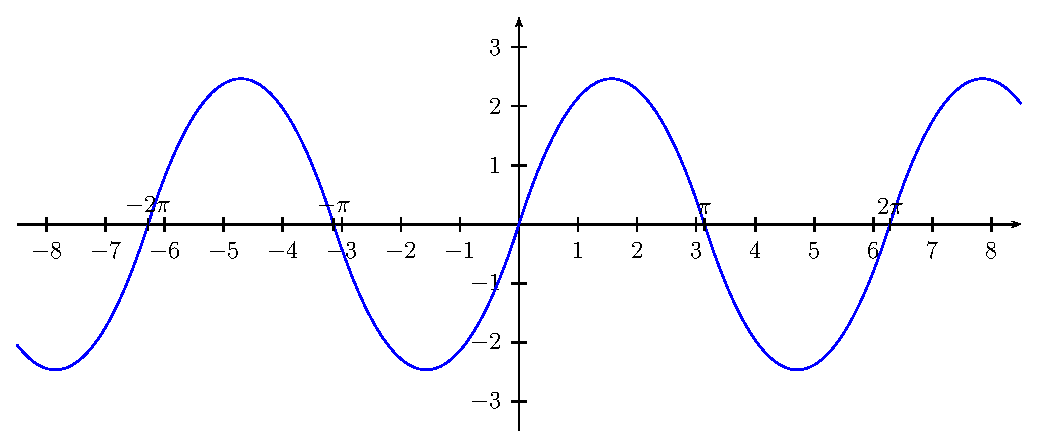
\includegraphics{../images/img005782-2}$$



Puisque $f$ est impaire, $\forall n\in\Nn$, $a_n(f)=0$ puis pour $n\in\Nn^*$, 

\begin{align*}\ensuremath
b_n(f)&=\frac{2}{\pi}\int_{0}^{\pi}x(\pi-x)\sin(nx)\;dx=\frac{2}{\pi}\left(\left[x(\pi-x)\frac{-\cos(nx)}{n}\right]_0^\pi+\frac{1}{n}\int_{0}^{\pi}(\pi-2x)\cos(nx)\;dx\right)\\
 &=\frac{2}{n\pi}\left(\left[(\pi-2x)\frac{\sin(nx)}{n}\right]_0^\pi+\frac{2}{n}\int_{0}^{\pi}\sin(nx)\;dx\right)=\frac{4}{n^2\pi}\left[-\frac{\cos(nx)}{n}\right]_0^\pi=\frac{4(1-(-1)^n)}{n^3\pi}.
\end{align*} 

La fonction $f$ est $2\pi$-périodique, continue sur $\Rr$ et de classe $C^1$ par morceaux sur $\Rr$. D'après le théorème de \textsc{Dirichlet}, la série de \textsc{Fourier} de $f$ converge vers $f$ sur $\Rr$. Par suite, pour tout réel $x$, 

\begin{center}
$f(x)=\frac{a_0(f)}{2}+\sum_{n=1}^{+\infty}(a_n(f)\cos(nx)+b_n(f)\sin(nx))=\frac{4}{\pi}\sum_{n=1}^{+\infty}\frac{1-(-1)^n}{n^3}\sin(nx)=\frac{8}{\pi}\sum_{p=0}^{+\infty}\frac{\sin((2p+1)x)}{(2p+1)^3}$.
\end{center}

\begin{center}
\shadowbox{
$\forall x\in\Rr$, $f(x)=\frac{8}{\pi}\sum_{n=0}^{+\infty}\frac{\sin((2n+1)x)}{(2n+1)^3}$.
}
\end{center}

L'égalité $f\left(\frac{\pi}{2}\right)=\frac{\pi^2}{4}$ fournit $\sum_{n=0}^{+\infty}(-1)^n\frac{1}{(2n+1)^3}=\frac{\pi^3}{32}$. Ensuite,  puisque $f$ est continue par morceaux sur $\Rr$ et $2\pi$-périodique, la formule de \textsc{Parseval} fournit $\frac{(a_0(f))^2}{2}+\sum_{n=1}^{+\infty}((a_n(f))^2+(b_n(f))^2)=\frac{1}{\pi}\int_{-\pi}^{\pi}(f(x))^2\;dx$ et donc

\begin{center}
$\frac{64}{\pi^2}\sum_{n=0}^{+\infty}\frac{1}{(2n+1)^6}=\frac{2}{\pi}\int_{0}^{\pi}x^2(\pi-x)^2\;dx=\frac{2}{\pi}\left[\pi^2\frac{x^3}{3}-2\pi\frac{x^4}{4}+\frac{x^5}{5}\right]_0^\pi=2\pi^4\left(\frac{1}{3}-\frac{1}{2}+\frac{1}{5}\right)=\frac{\pi^4}{15}$
\end{center}

et donc $\sum_{n=0}^{+\infty}\frac{1}{(2n+1)^6}=\frac{\pi^2}{64}\times\frac{\pi^4}{15}=\frac{\pi^6}{960}$. Enfin, si on pose $S=\frac{1}{n^6}$,

\begin{center}
$S=\sum_{n=0}^{+\infty}\frac{1}{(2n+1)^6}+\sum_{n=1}^{+\infty}\frac{1}{(2n)^6}=\frac{\pi^6}{960}+\frac{S}{64}$,
\end{center}

et donc $S=\frac{64}{63}\times\frac{\pi^6}{960}=\frac{\pi^6}{945}$.

\begin{center}
\shadowbox{
$\sum_{n=0}^{+\infty}(-1)^n\frac{1}{(2n+1)^3}=\frac{\pi^3}{32}$, $\sum_{n=1}^{+\infty}\frac{1}{(2n+1)^6}=\frac{\pi^6}{960}$ et $\sum_{n=1}^{+\infty}\frac{1}{n^6}=\frac{\pi^6}{945}$.
}
\end{center}
La fonction $f$ est continue par morceaux sur $\Rr$ et $2\pi$-périodique. On peut donc calculer ses coefficients de \textsc{Fourier}.

$$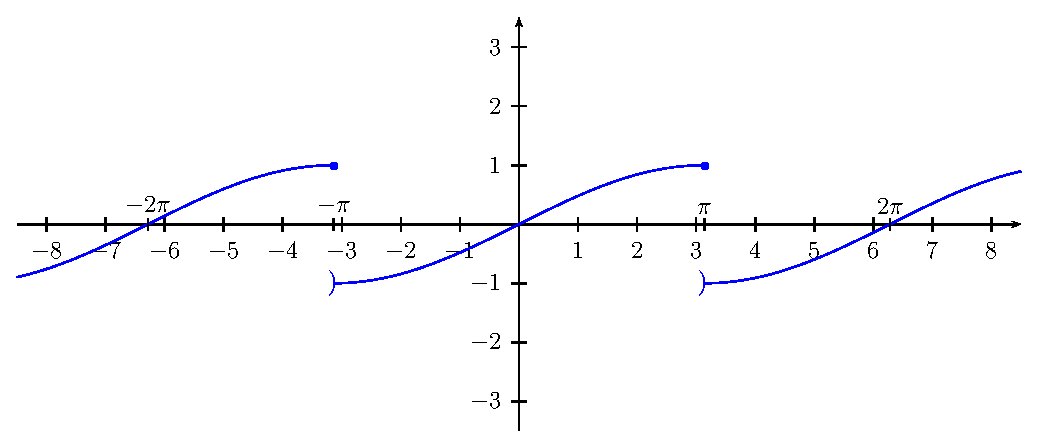
\includegraphics{../images/img005782-3}$$


La fonction $f$ a mêmes coefficients de \textsc{Fourier} que la fonction $g$ définie sur $\Rr$, impaire et $2\pi$-périodique telle que $\forall x\in\left]0,\frac{\pi}{2}\right[$, $g(x)=0$. Donc $\forall n\in\Nn$, $a_n(f)=0$ puis pour $n\in\Nn^*$,

\begin{align*}\ensuremath
b_n(f)&=\frac{2}{\pi}\int_{0}^{\pi}\sin\left(\frac{x}{2}\right)\sin(nx)\;dx=\frac{1}{\pi}\int_{0}^{\pi}\left(\cos\left(\left(n-\frac{1}{2}\right)x\right)-\cos\left(\left(n+\frac{1}{2}\right)x\right)\right)dx\\
 &=\frac{1}{\pi}\left[\frac{\sin\left(\left(n-\frac{1}{2}\right)x\right)}{n-\frac{1}{2}}-\frac{\sin\left(\left(n+\frac{1}{2}\right)x\right)}{n+\frac{1}{2}}\right]_0^\pi=\frac{1}{\pi}\left(-\frac{(-1)^n}{n-\frac{1}{2}}-\frac{(-1)^n}{n+\frac{1}{2}}\right)\\
 &=-\frac{(-1)^n}{\pi}\frac{2n}{n^2-\frac{1}{4}}=-\frac{(-1)^n}{\pi}\frac{8n}{4n^2-1}.
\end{align*}

La fonction $f$ est $2\pi$-périodique et de classe $C^1$ par morceaux sur $\Rr$. D'après le théorème de \textsc{Dirichlet}, la série de \textsc{Fourier} de $f$ converge en tout réel $x$ et a pour somme $\frac{1}{2}(f(x^+)+f(x^-)$. En particulier,

\begin{center}
\shadowbox{
$\forall x\in]-\pi,\pi[$, $\sin\left(\frac{x}{2}\right)=-\frac{8}{\pi}\sum_{n=1}^{+\infty}(-1)^n\frac{n}{4n^2-1}\sin(nx)$.
}
\end{center}

L'égalité $f\left(\frac{\pi}{2}\right)=\frac{1}{\sqrt{2}}$ fournit 

\begin{center}
$\frac{1}{\sqrt{2}}=-\frac{8}{\pi}\sum_{n=0}^{+\infty}(-1)^n\frac{n}{4n^2-1}\sin\left(n\frac{\pi}{2}\right)=\frac{8}{\pi}\sum_{p=0}^{+\infty}\frac{2p+1}{4(2p+1)^2-1}\sin\left((2p+1)\frac{\pi}{2}\right)=\frac{8}{\pi}\sum_{p=0}^{+\infty}(-1)^p\frac{2p+1}{16p^2+1p+3}$,
\end{center}

\begin{center}
\shadowbox{
$\sum_{n=0}^{+\infty}(-1)^n\frac{2n+1}{16n^2+16n+3}=\frac{\pi}{8\sqrt{2}}$.
}
\end{center}
$f$ est $2\pi$-périodique, continue par morceaux sur $\Rr$ et paire. Pour $n\in\Nn^*$, $b_n(f)=0$ puis pour $n\in\Nn$, $a_n(f)=\frac{1}{\pi}\int_{-\pi}^{\pi}\ch(\lambda x)\cos(nx)\;dx$.

\textbf{1ère solution.} Soit $n\in\Nn$.

\begin{align*}\ensuremath
a_n(f)&=\frac{1}{\pi}\text{Re}\left(\int_{-\pi}^{\pi}\ch(\lambda x)e^{inx}\;dx\right)=\frac{1}{2\pi}\text{Re}\left(\int_{-\pi}^{\pi}e^{(\lambda+in)x}\;dx+\int_{-\pi}^{\pi}e^{(-\lambda+in)x}\;dx\right)\\
 &=\frac{1}{2\pi}\text{Re}\left(\frac{e^{(\lambda+in)\pi}-e^{-(\lambda+in)\pi}}{\lambda+in}+\frac{e^{(-\lambda+in)\pi}-e^{-(-\lambda+in)\pi}}{-\lambda+in}\right)=\frac{(-1)^n}{2\pi}\text{Re}\left(\frac{2\sh(\lambda\pi)}{\lambda+in}+\frac{-2\sh(\lambda\pi)}{-\lambda+in}\right)\\
 &=\frac{(-1)^n\sh(\lambda\pi)}{\pi}\text{Re}\left(\frac{\lambda-in}{\lambda^2+n^2}+\frac{\lambda+in}{\lambda^2+n^2}\right)=\frac{2\lambda\sh(\lambda\pi)}{\pi}\times\frac{(-1)^n}{n^2+\lambda^2}
\end{align*}

\textbf{2ème solution.} Une double intégration par parties fournit

\begin{align*}\ensuremath
a_n(f)&=\frac{1}{\pi}\left(\left[\frac{\sh(\lambda x)}{\lambda}\cos(nx)\right]_{-\pi}^{\pi}+\frac{n}{\lambda}\int_{-\pi}^{\pi}\sh(\lambda x)\sin(nx)\;dx\right)=\frac{1}{\pi}\left(\frac{2(-1)^n\sh(\lambda\pi)}{\lambda}+\frac{n}{\lambda}\int_{-\pi}^{\pi}\sh(\lambda x)\sin(nx)\;dx\right)\\
 &=\frac{1}{\pi}\left(\frac{2(-1)^n\sh(\lambda\pi)}{\lambda}+\frac{n}{\lambda}\left(\left[\frac{\ch(\lambda x)}{\lambda}\sin(nx)\right]_{-\pi}^{\pi}-\frac{n}{\lambda}\int_{-\pi}^{\pi}\ch(\lambda x)\cos(nx)\;dx\right)\right)\\
 &=\frac{2(-1)^n\sh(\lambda\pi)}{\lambda\pi}-\frac{n^2}{\lambda^2}a_n(f),
\end{align*}

et donc $\forall n\in\Nn$, $a_n(f)=\frac{2(-1)^n\sh(\lambda\pi)}{\lambda\pi}\times\frac{\lambda^2}{n^2+\lambda^2}=\frac{2\lambda\sh(\lambda\pi)}{\pi}\times\frac{(-1)^n}{n^2+\lambda^2}$.

La fonction $f$ est $2\pi$-périodique, continue sur $\Rr$ et de classe $C^1$ par morceaux sur $\Rr$. D'après le théorème de \textsc{Dirichlet}, la série de \textsc{Fourier} de $f$ converge vers $f$ sur $\Rr$. On en déduit que

\begin{center}
\shadowbox{
$\forall x\in\Rr$, $f(x)=\frac{\sh(\lambda\pi)}{\lambda\pi}+\frac{2\lambda\sh(\lambda\pi)}{\pi}\sum_{n=1}^{+\infty}\frac{(-1)^n}{n^2+\lambda^2}\cos(nx)$.
}
\end{center}

L'égalité $f(0)=1$ fournit $1=\frac{\sh(\lambda\pi)}{\lambda\pi}+\frac{2\lambda\sh(\lambda\pi)}{\pi}\sum_{n=1}^{+\infty}\frac{(-1)^n}{n^2+\lambda^2}$ et donc

\begin{center}
$\sum_{n=1}^{+\infty}\frac{(-1)^n}{n^2+\lambda^2}=\frac{\pi}{2\lambda\sh(\lambda\pi)}\left(1-\frac{\sh(\lambda\pi)}{\lambda\pi}\right)=\frac{\pi\left(\sh(\lambda\pi)-\pi\lambda\right)}{2\lambda^2\pi\sh(\lambda\pi)}$
\end{center}

et l'égalité $f(\pi)=\ch(\lambda\pi)$ fournit 

\begin{center}
$\sum_{n=1}^{+\infty}\frac{1}{n^2+\lambda^2}=\frac{\pi}{2\lambda\sh(\lambda\pi)}\left(\ch(\lambda\pi)-\frac{\sh(\lambda\pi)}{\lambda\pi}\right)=\frac{\lambda\pi\ch(\lambda\pi)-\sh(\lambda\pi)}{2\lambda^2\sh(\lambda\pi)}$
\end{center}

\begin{center}
\shadowbox{
$\forall\lambda>0$, $\sum_{n=1}^{+\infty}\frac{(-1)^n}{n^2+\lambda^2}=\frac{\pi}{2\lambda\sh(\lambda\pi)}$ et $\sum_{n=1}^{+\infty}\frac{1}{n^2+\lambda^2}=\frac{\lambda\pi\ch(\lambda\pi)-\sh(\lambda\pi)}{2\lambda^2\sh(\lambda\pi)}$.
}
\end{center}

La fonction $f$ est $2\pi$-périodique, continue par morceaux sur $\Rr$. L'égalité de \textsc{Parseval} s'écrit $\frac{(a_0(f))^2}{2}+\sum_{n=1}^{+\infty}((a_n(f))^2+(b_n(f))^2)=\frac{1}{\pi}\int_{-\pi}^{\pi}(f(x))^2\;dx$ avec

\begin{center}
$\frac{1}{\pi}\int_{-\pi}^{\pi}(f(x))^2\;dx=\frac{1}{\pi}\int_{-\pi}^{\pi}\ch^2(\lambda x)\;dx=\frac{1}{\pi}\int_{-\pi}^{\pi}\frac{\ch(2\lambda x)+1}{2}\;dx=1+\frac{\sh(2\lambda\pi)}{2\pi}$,
\end{center}

et donc $1+\frac{\sh(2\lambda\pi)}{2\pi}=\frac{2\sh^2(\lambda\pi)}{\pi^2\lambda^2}+\frac{4\lambda^2\sh^2(\lambda\pi)}{\pi^2}\sum_{n=1}^{+\infty}\frac{1}{(\lambda^2+n^2)^2}$ puis

\begin{center}
$\sum_{n=1}^{+\infty}\frac{1}{(\lambda^2+n^2)^2}=\frac{\pi^2}{4\lambda^2\sh^2(\lambda\pi)}\left(1+\frac{\sh(2\lambda\pi)}{2\pi}-\frac{2\sh^2(\lambda\pi)}{\pi^2\lambda^2}\right)=\frac{2\pi^2\lambda^2+\pi\lambda\sh(2\lambda\pi)-4\lambda^2\sh^2(\lambda\pi)}{8\lambda^4\sh^2(\lambda\pi)}$.
\end{center}

\begin{center}
\shadowbox{
$\forall\lambda>0$, $\sum_{n=1}^{+\infty}\frac{1}{(\lambda^2+n^2)^2}=\frac{\pi^2\lambda^2+\pi\lambda\ch(\lambda\pi)\sh(\lambda\pi)-2\lambda^2\sh^2(\lambda\pi)}{4\lambda^2\sh^2(\lambda\pi)}$.
}
\end{center}
La fonction $f$ est continue par morceaux sur $\Rr$ et $2\pi$-périodique. On peut donc calculer ses coefficients de \textsc{Fourier}.

$$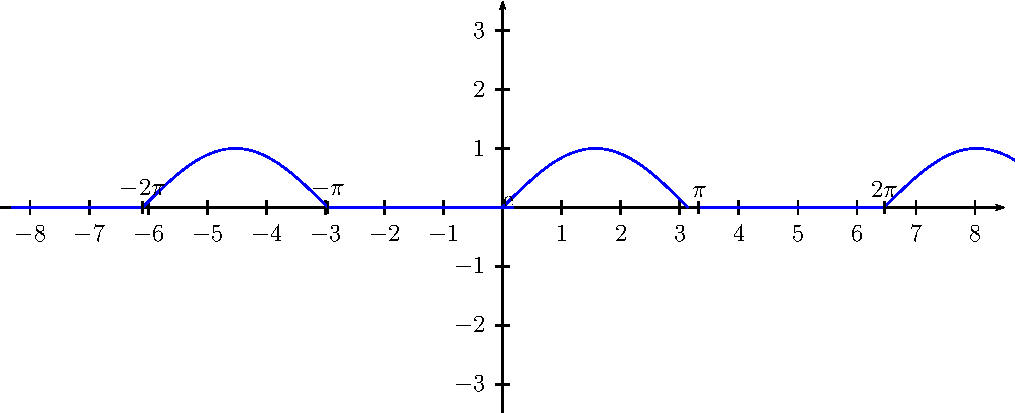
\includegraphics{../images/img005782-4}$$


Soit $n\in\Nn$.

\begin{align*}\ensuremath
a_n(f)&=\frac{1}{\pi}\int_{-\pi}^{\pi}\text{sup}(\sin x,0)\cos(nx)\;dx=\frac{1}{\pi}\int_{0}^{\pi}\sin x\cos(nx)\;dx=\frac{1}{2\pi}\int_{0}^{\pi}\sin((n+1)x)-\sin((n-1)x)\;dx\\
 &=\left\{
 \begin{array}{l}
 \frac{1}{2\pi}\int_{0}^{\pi}\sin(2x)\;dx\;\text{si}\;n=1\\
 \frac{1}{2\pi}\left[-\frac{\cos((n+1)x)}{n+1}+\frac{\cos((n-1)x)}{n-1}\right]_0^\pi\;\text{si}\;n\neq1
 \end{array}
 \right.=\left\{
 \begin{array}{l}
 \frac{1}{2\pi}\left[-\frac{\cos(2x)}{2}\right]_0^\pi\;\text{si}\;n=1\\
 \frac{1}{2\pi}\left(-\frac{(-1)^{n+1}-1}{n+1}+\frac{(-1)^{n-1}-1}{n-1}\right)\;\text{si}\;n\neq1
 \end{array}
 \right.\\
 &=\left\{
 \begin{array}{l}
\rule[-2mm]{0mm}{0mm}0\;\text{si}\;n=1\\
-\frac{1+(-1)^n}{\pi}\frac{1}{n^2-1}\;\text{si}\;n\neq1
 \end{array}
 \right.
\end{align*}

Soit $n\in\Nn^*$.

\begin{align*}\ensuremath
b_n(f)&=\frac{1}{\pi}\int_{0}^{\pi}\sin x\sin(nx)\;dx=\frac{1}{2\pi}\int_{0}^{\pi}(\cos((n-1)x)-\cos((n+1)x))\;dx=\left\{
 \begin{array}{l}
 \frac{1}{2}\;\text{si}\;n=1\\
\rule{0mm}{4mm} 0\;\text{si}\;n\neq1
 \end{array}
 \right.\end{align*}

La fonction $f$ est $2\pi$-périodique, continue sur $\Rr$ et de classe $C^1$ par morceaux sur $\Rr$. D'après le théorème de \textsc{Dirichlet}, la série de \textsc{Fourier} de $f$ converge vers $f$ sur $\Rr$. On en déduit que pour tout réel $x$

\begin{center}
$\text{sup}(\sin x,0)=\frac{1}{\pi}+\frac{\sin x}{2}-\frac{1}{\pi}\sum_{n=2}^{+\infty}\frac{1+(-1)^n}{n^2-1}\cos(nx)=\frac{1}{\pi}+\frac{\sin x}{2}-\frac{2}{\pi}\sum_{p=1}^{+\infty}\frac{1}{4p^2-1}\cos(2px)$.
\end{center}

\begin{center}
\shadowbox{
$\forall x\in\Rr$, $\text{sup}(\sin x,0)=\frac{1}{\pi}+\frac{\sin x}{2}-\frac{2}{\pi}\sum_{n=1}^{+\infty}\frac{1}{4n^2-1}\cos(2nx)$.
}
\end{center}

L'égalité $f(0)=0$ fournit $\frac{1}{\pi}-\frac{2}{\pi}\sum_{n=1}^{+\infty}\frac{1}{4n^2-1}=0$ et donc

\begin{center}
\shadowbox{
$\sum_{n=1}^{+\infty}\frac{1}{4n^2-1}=\frac{1}{2}$.
}
\end{center}

\textbf{Remarque.} $\sum_{n=1}^{+\infty}\frac{1}{4n^2-1}=\lim_{N \rightarrow +\infty}\frac{1}{2}\sum_{n=1}^{N}\left(\frac{1}{2n-1}-\frac{1}{2n+1}\right)=\lim_{N \rightarrow +\infty}\frac{1}{2}\left(1-\frac{1}{2N+1}\right)=\frac{1}{2}$
}
}
